\section{Durchführung}
\label{sec:Durchführung}
\begin{figure}
  \centering
  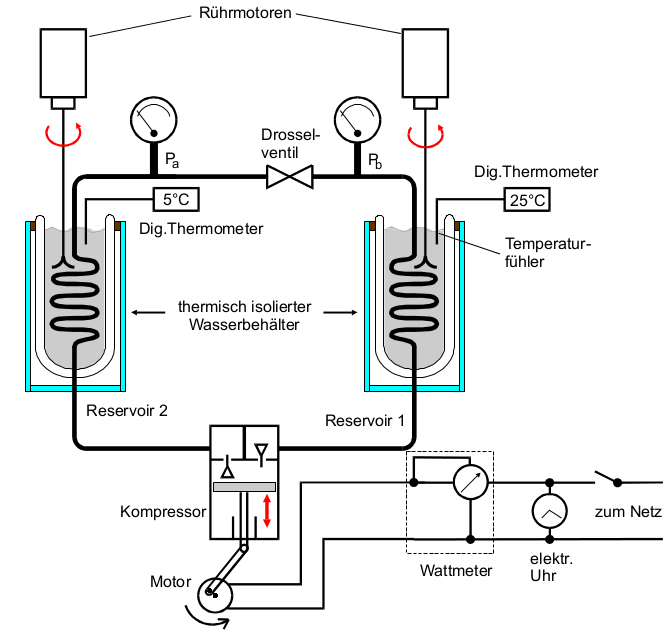
\includegraphics[width=0.60\textwidth]{messapparatur.png}
  \caption{Aufbau der Messapparatur.}
  \label{fig:aufbau}
\end{figure}
Zu Beginn werden die Reservoire 1 und 2 mit je drei Litern Wasser gefüllt. Um die
Menge genau messen zu können, wird ein Messkolben mit einem Fassungsvolumen von
einem Liter verwendet.
Es werden der Kompressor und die Rührmotoren, die dafür sorgen, dass die Temperatur in
den Behältern immer gleichmäßig verteilt ist, angeschaltet.
Nun werden im Abstand von einer Minute die Temperaturen $T_1$ und $T_2$, die Drücke
$p_\symup{a}$ und $p_\symup{b}$, sowie die Leistungsaufnhame $N$ des Kompressors
abgelesen. Dies wird solange wiederholt, bis die Temperatur $T_1$ 50°C erreicht hat.
Da die Manometer bei Umgebungsdruck auf 0 Bar geeicht sind, muss auf alle abgelesenen
Drücke 1 Bar addiert werden.
